\mode*
\mode<all>{\topsection{Niezmienniki krzywych}}
Często możemy zauważyć, że krzywa w jednym punkcie ,,krzywi" się bardziej, niż innym. Typowym przykładem może być wykres funkcji $f(x)=x^2$ i porównanie jego zachowania się w pobliżu punktu $(0,0)$ z punktem powiedzmy $(3,9)$. Chcemy tę intuicyjną różnicę wyrazić w sposób ścisły.

Jeśli przyjmiemy, że prosta się nie ,,krzywi'', wtedy nasza domniemana definicja \textit{krzywizny} powinna określać w każdym punkcie jak bardzo nasza krzywa $\alpha\colon (a,b)\to \R^3$ (lokalnie, tj. w małym otoczeniu każdego punktu) różni się właśnie od prostej. Tak więc krzywizna będzie będzie pewną funkcją (gładką) $\kappa\colon (a,b)\to \R$ która będzie przyjmować dla $t_0\in (a,b)$ wartość $0$ jeśli tylko wykres krzywej w małym otoczeniu $t_0$ będzie linią prostą.

Rozwazmy wektor prędkości dla krzywej $\alpha$. Im szybciej zmienia on kierunek, tym bardziej nasza krzywa wydaje się ,,krzywić". Zatem definicja krzywizny powinna być związana z wektorem pochodnych wektora prędkości. Oczywiście natychmias pojawia się problem zależności takich definicji od parametryzacji. Jeśli weźmiemy reparametryzację krzywej $\alpha$ która przebiega obraz szybciej, wtedy niejako \textit{z definicji} okaże się że kierunek wektora stycznego zmienia się szybciej.
Aby obejść tę trudność zaczniemy od krzywizny dla krzywych unormowanych.

\mode<all>{\midsection{Krzywizna}}
\begin{frame}{Krzywizna krzywej unormowanej}
\begin{definicja}
Niech $\alpha\colon(a,b)\to \R^3$ będzie (regularną) krzywą unormowaną. Dla każdego $t\in (a,b)$ \textbf{krzywiznę} definiujemy jako funkcję $\kappa\colon (a,b)\to\R$
\[\kappa(t)\define\|T\,'(t)\|=\|\alpha''(t)\|\]
Zauważmy, że krzywizna jest zawsze nieujemna, $\kappa(t)\geqslant 0$.
\end{definicja}
\end{frame}
%%%%%%next-slide%%%%%
\begin{frame}
\begin{center}
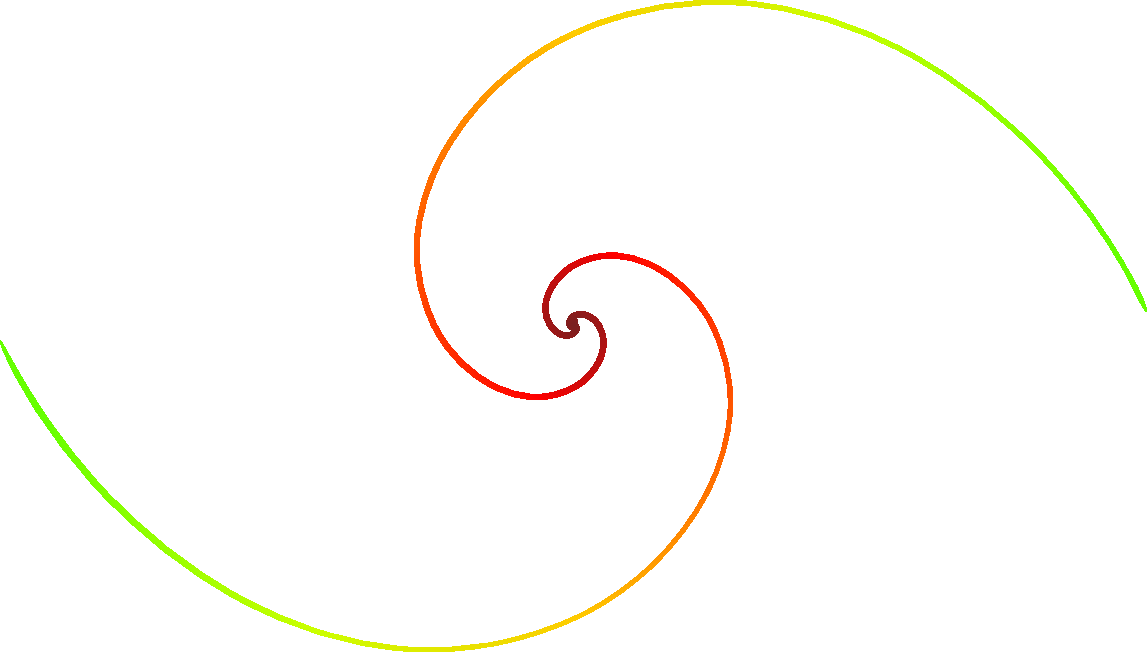
\includegraphics[scale=.5]{./pictures/curvature_color.pdf}\\

Zmiana koloru w zależności od krzywizny
\end{center}
\end{frame}
%%%%%%next-slide%%%%%
\begin{frame}{Krzywizna dowolnej krzywej}

Dla regularnych krzywych nieunormowanych możemy posłużyć się odpowiednią reparametryzacją:
\pause \begin{definicja}
Niech $\alpha\colon (a,b)\to \R^3$ będzie krzywą regularną, oraz niech $\beta=\alpha\circ h \colon (c,d)\to \R^3$ będzie jej reparametryzacją unormowaną ($h\colon (c,d)\to (a,b)$). Wówczas \[\kappa_\alpha(t)\define\kappa_\beta(h^{-1} (t)\!)\]
\end{definicja}

\pause\mode<presentation>{Czy definicja jest niezależna od wyboru parametryzacji?}

\end{frame}
%%%%%%next-slide%%%%%
Taka definicja rodzi natychmiast pytanie o jednoznaczność definicji krzywizny, ponieważ potencjalnie różne reparametryzacje unormowane mogą prowadzić do różnych funkcji krzywizny. Mamy jednak następujący lemat.

\begin{frame}[<+->]
\begin{lemat}
Niech $\alpha\colon(a,b)\to \R^3$ będzie krzywą regularną i niech $\alpha\circ h_1$ oraz $\alpha\circ h_2$ będą dwiema reparametryzacjami unormowanymi, gdzie $h_1\colon (c_1,d_1)\to (a,b)$, oraz $h_2\colon (c_2,d_2)\to (a,b)$ są dyfeomorfizmami. Jeśli $\kappa_1$ i $\kappa_2$ oznaczają krzywizny krzywych odpowiednio $\alpha\circ h_1$ oraz $\alpha\circ h_2$, wtedy\[\kappa_1(h_1^{-1}(t))=\kappa_2(h_2^{-1}(t))\]
dla wszystkich $t\in (a,b)$.

\end{lemat}

\begin{wniosek}
Definicja krzywizny dla krzywej nieunormowanej nie zależy od wyboru parametryzacji.
\end{wniosek}

\end{frame}
%%%%%%next-slide%%%%%
\begin{frame}[<+->]

\textcolor{ared}{\textbf{Dowód:}}\pause \\
Najpierw pokażemy, że $h_1$ i $h_2$ (funkcje reparametryzujące do krzywych unormowanych) mogą się różnić jedynie znakiem i przesunięciem, \pause tj. pokażemy, że złożenie \[h_2^{-1}\circ h_1\colon (c_1,d_1)\to (c_2,d_2)\] jest równe \[\left(h_2^{-1}\circ h_1\right)(t)=\pm t+C,\] dla pewnej stałej $C\in \R$.

\pause Dla obu indeksów $i=1,2$ i wszystkich $t\in (c_i,d_i)$ mamy 
\[1=\|(\alpha\circ h_i)'(t)\|=\|\alpha'(h_i(t))\||h'_i(t)|.\]
\end{frame}
%%%%%%next-slide%%%%%
\begin{frame}[<+->]

Zatem dla wszystkich $t\in (c_1,d_1)$ zachodzi 
\mode<article>{
\begin{multline*}
h_1'(t)=\frac{\pm1}{\|\alpha'(h_1(t))\|}=
\frac{\pm1}{\left\|\alpha'\left(h_2\left(h_2^{-1}\left[h_1(t)\right]
\right)\right)\right\|}=\pause\pm 
h_2\left[\left(h_2^{-1}\circ 
h_1\right)\!(t)\right]\!\!.
\end{multline*}}
\mode<presentation>{
\begin{multline*}
h_1'(t)=\frac{\pm1}{\|\alpha'(h_1(t))\|}=
\frac{\pm1}{\left\|\alpha'\left(h_2\left(h_2^{-1}\left[h_1(t)\right]
\right)\right)\right\|}=\\\pause=\pm 
h_2\left[\left(h_2^{-1}\circ 
h_1\right)\!(t)\right]\!\!.
\end{multline*}}

\pause Możemy teraz policzyć pochodną funkcji wewnętrznej:
\[
(h_2^{-1}\circ h_1)'(t)=\left(h_2^{-1}\right)'\big[h_1(t)\big]h_1'(t)=\frac{h_1'(t)}{h_2'(h_2^{-1}\circ h_1(t))}=\pm 1
\]

\pause Całkując obie strony równości otrzymujemy
\begin{align*}
\onslide<4->{\left(h_2^{-1}\circ h_1\right)(t)=}&\onslide<4->{\pm t+C\\}
\onslide<5->{h_1(t)=}&\onslide<5->{h_2(\pm t+C)\\}
\onslide<6->{h_2^{-1}(t)=}&\onslide<6->{h_1^{-1}(\pm t)+C.}
\end{align*}
\end{frame}
%%%%%%next-slide%%%%%
\begin{frame}[<+->]


Podstawiając przedostatnią równość do $\alpha$ mamy 
\[(\alpha\circ h_1)(t)=(\alpha\circ h_2)(\pm t+C),\]
\pause więc zachodzi również $\kappa_1(t)=\kappa_2(\pm t+C)$. \pause Podstawiając teraz $t=h_1^{-1}(s)$ otrzymujemy 
\[\kappa_1(h_1^{-1})(s)=\kappa_2(h_1^{-1}(s)+C)=\kappa_2(h_2^{-1}(s)\!).\]
\hfill $\square$

\end{frame}
%%%%%%next-slide%%%%%

\begin{uwaga}
Na razie pokazaliśmy, że dla \textit{wybranej} parametryzacji $\alpha$ krzywizna 
nie zależy od reparametryzacji unormowanej.

Chcemy jednak pokazać coś więcej, mianowicie, że krzywizna jest funkcją zależną tylko od \textit{punktów w obrazie krzywej} i w ogóle nie zależy od wyboru \textit{parametryzacji}. Zostanie to wykazane pod koniec tego wykładu.
\end{uwaga}


%%%%%%next-slide%%%%%
\begin{frame}

\begin{lemat}
Niech $\alpha\colon (a,b)\to \R^3$ będzie krzywą regularną. Wektor normalny do $\alpha$ jest zerowy wtedy i tylko wtedy, gdy $\alpha$ jest prostą.
\end{lemat}
\pause\textcolor{ared}{\textbf{Dowód:}}\\
Bez straty ogólności możemy założyć, że $\alpha$ jest krzywą unormowaną.
\pause Załóżmy, że wektor normalny do $\alpha$ jest zerowy, \[\frac{T'(t)}{|T'(t)|}=N(t)=(0,0,0).\] \pause 
Całkując to równanie otrzymujemy 
 \begin{multline*}
T(t)=\int T'(t)\,dt=\left(\int T_1 '(t)\,dt,\int T_2 '(t)\,dt, \int T_3 '(t)\,dt\right)=\pause\\=\left(\int 0\,dt,\int 0\,dt, \int 0\,dt\right)=(c_1,c_2,c_3)=v=\text{\footnotesize{const}}.
\end{multline*}


\end{frame}
%%%%%%next-slide%%%%%
\begin{frame}[<+->]
Całkując ponownie mamy \[\alpha(t)=vt+w,\] gdzie $v,w\in \R^3$ są ustalonymi wektorami, czyli $\alpha$ jest prostą.
\pause 
Załóżmy teraz, że $\alpha$ jest prostą. \pause Mamy wtedy (postać parametryczna prostej) $\alpha(t)=vt+w$, gdzie $v,w\in \R^3$. \pause Wtedy oczywiście \[T(t)=\frac{\alpha'(t)}{\|\alpha'(t)\|}=\frac{v}{\|v\|},\] zatem $T\,'(t)=0$ więc automatycznie $N(t)=0$.
\hfill $\square$

\end{frame}
%%%%%%next-slide%%%%%
\mode<all>{\midsection{Torsja}}
\begin{frame}
\begin{definicja}
Niech $\alpha\colon (a,b)\to \R^3$ będzie krzywą regularną, oraz załóżmy, że dla wszystkich $t\in (a,b)$ zachodzi $N(t)\neq 0$. \textbf{Torsję} krzywej $\alpha$ w punkcie $t$ definiujemy jako funkcję \[\tau(t)\define \langle B'(t),N(t)\rangle.\]
\end{definicja}
\pause
\begin{uwaga}
\begin{itemize}
\item Torsja jest funkcją gładką (wynika to z gładkości iloczynu skalarnego).
\pause\item Podobnie jak w przypadku krzywizny mamy $|\tau(t)|=\|B'(t)\|$, 
jednak torsja może mieć wartości \textit{ujemne}.
\end{itemize}
\end{uwaga}

\end{frame}
%%%%%%next-slide%%%%%
\begin{frame}[<+->]

\begin{uwaga}
Dla wygody od teraz będziemy opuszczać argument $t$ jeśli nie będzie to prowadziło do niejednoznaczności.
\end{uwaga}

\end{frame}
%%%%%%next-slide%%%%%
\mode<all>{\midsection{Wzory Freneta}}
\begin{frame}
\begin{twierdzenie}[Wzory Freneta] Niech $\alpha\colon (a,b)\to \R^3$ będzie unormowaną krzywą regularną, r\'ożną od stałej i prostej (tj. $N(t)\neq 0$ dla wszystkich $t\in (a,b)$). Wówczas zachodzą następujące równości.
\begin{align}
T\,'	&= \qquad\kappa N \label{eqn:frenet1} \\
N\hspace{0.5pt}'	&= -\kappa T + \tau B\label{eqn:frenet2}\\
B'	&= \quad-\tau N\label{eqn:frenet3}
\end{align}
\pause co można zapisać w postaci wektorowej
\[
\left(\begin{array}{c}
 T\\
 N\\
 B
 \end{array}\right)'=
 \left[\begin{array}{r r r}
 0 & \kappa & 0\\
 -\kappa & 0 & \tau\\
 0 & -\tau &0
 \end{array}\right]
 \left(\begin{array}{c}
  T\\
 N\\
 B
 \end{array}\right)
\]


\end{twierdzenie}

\end{frame}
%%%%%%next-slide%%%%%
\begin{frame}

\textcolor{ared}{\textbf{Dowód:}}\pause \\
Wzór \ref{eqn:frenet1} na $T\,'$ wynika z przyjętych definicji $\kappa$ i $N$.

\pause Ponieważ wektory z repera Freneta są jednostkowe, więc $N\hspace{0.5pt}'$ jest prostopadły do $N$. Ponieważ jednak ${T,N,B}$ tworzy bazę przestrzeni $\R^3$, więc $N\hspace{0.5pt}'$ musi być kombinacją liniową wektorów $T$ i $B$,\[N\hspace{0.5pt}'=a T+b B.\] 
\pause Mnożąc tę równość skalarnie przez wektor $T$ (odpowiednio $B$) otrzymujemy $a=\langle N\hspace{0.5pt}',T\hspace{0.5pt}\rangle$ (odpowiednio $b=\langle N\hspace{0.5pt}',B\rangle$). \pause Wyliczenie $a$ rozpocznijmy od równości $0=\langle N,T\hspace{0.5pt}\rangle$. Różniczkując obie strony otrzymujemy
\pause \[0=\langle N\hspace{0.5pt}',T\hspace{0.5pt}\rangle+\langle N,T\,'\rangle=\langle N\hspace{0.5pt}',T\hspace{0.5pt}\rangle+\underbrace{\langle N,\kappa N\rangle}_{=\kappa},\]
\pause zatem $a=\langle N\hspace{0.5pt}',T\hspace{0.5pt}\rangle=-\kappa$. \pause Ponieważ $\langle N,B\rangle=0$, w podobny sposób możemy stwierdzić, że $\langle N\hspace{0.5pt}',B\rangle=-\tau$. Pozostawiamy to jako zadanie domowe.

\end{frame}
%%%%%%next-slide%%%%%
\begin{frame}[<+->]
Podobnie $B'$ jest prostopadły do $B$, $\langle B,B'\rangle=0$, więc
\[B'=a T+b N.\]
\pause Musimy więc policzyć $a=\langle B',T\hspace{0.5pt}\rangle$ i $b=\langle B',N\rangle$. Wyliczenie $a$ rozpocznijmy od równości: $0=\langle B,T\hspace{0.5pt}\rangle$. \pause Różniczkując obie strony otrzymujemy
\[0=\langle B',T\hspace{0.5pt}\rangle+\langle B,T\,'\rangle=\langle B',T\hspace{0.5pt}\rangle+\langle B,\kappa N\rangle=\langle B',T\hspace{0.5pt}\rangle.\]
\pause Tak więc $B'$ jest współliniowy z $N$ i równość \ref{eqn:frenet3} charakteryzująca $B'$ wynika z definicji torsji $\tau$.

\hfill $\square$

\end{frame}
%%%%%%next-slide%%%%%
\begin{frame}[<+->]

\begin{lemat}
Niech $\alpha\colon (a,b)\to \R^3$ będzie krzywą unormowaną oraz niech $N(t)\neq 0$ dla każdego $t\in (a,b)$. Następujące warunki są równoważne.
\begin{enumerate}
\item Zbi\'or $\alpha(a,b)$ (tj. wykres $\alpha$) jest zawarty w pewnej płaszczyźnie.
\item $B$ jest wektorem stałym.
\item $\tau\equiv 0$.
\end{enumerate}

\end{lemat}

\begin{uwaga}
Krzywą spełniającą jeden z tych warunków nazywamy \textbf{krzywą płaską}.
\end{uwaga}

\end{frame}
%%%%%%next-slide%%%%%
\begin{frame}

\textcolor{ared}{\textbf{Dowód:}}\pause \\
\begin{description}
\item [$1\Rightarrow 2$] Jeśli krzywa leży w jednej płaszczyźnie to leżą w niej 
wektory styczny i normalny (dlaczego?), \pause więc jest to płaszczyzna ściśle 
styczna. \pause Wtedy kierunek prostopadły do tej płaszczyzny jest współliniowy 
z $B$. Zatem $B$ nie zmienia ani zwrotu ani długości.\pause
\item [$2\Leftrightarrow 3$] wynika ze wzoru Freneta (\ref{eqn:frenet3}):
\[B'=-\tau N\]
\end{description}

\end{frame}
%%%%%%next-slide%%%%%
\begin{frame}
\begin{description}
\item [$2\Rightarrow 1$] Niech $p\in (a,b)$ będzie punktem z dziedziny $\alpha$. 
\mode<presentation>{\begin{itemize}}
\mode<presentation>{\pause\item}
Rozważmy funkcję
\[f(t)=\langle \alpha(t)-\alpha(p),B(t)\rangle.\]

\mode<article>{
Funkcja ta mierzy długość rzutu wektora binormalnego na wektor wyznaczony przez naszą krzywą (bez straty ogólności możemy założyć, że $\alpha(p)=(0,0,0)$.)}

\mode<presentation>{\pause\item}
Przy założeniu, że $B(t)=B$ jest wektorem stałym, pokażemy, że funkcja $f$ jest tożsamościowo równa $0$, \pause z czego wynika, że krzywa $\alpha$ w całości leży w płaszczyźnie normalnej do $B$ i zawierającej punkt $\alpha(p)$.
\mode<presentation>{\end{itemize}}
\end{description}
\end{frame}
%%%%%%next-slide%%%%%
\begin{frame}
\mode<presentation>{\begin{itemize}}
\mode<presentation>{\item}
Obliczmy 
\[\begin{split}
f\,'(t)=&\pause\frac{d}{dt}\left(\langle\alpha(t)-\alpha(p),B(t)\rangle\right)=\\
\uncover<3->{=}&\uncover<3->{\underbrace{\langle\alpha'(t),B(t)\rangle}_{=\langle T(t),B(t)\rangle=0}+}
\uncover<4->{\underbrace{\langle\alpha(t)-\alpha(p),B'(t) \rangle}_{=0\text{ bo $B(t)$ jest stały}}=0.}
\end{split}\]
\uncover<5->{
\mode<presentation>{\item} Zatem $f$ jest funkcją stałą. Jeśli podstawimy $t=p$ otrzymamy $f(p)=0$, więc $f$ jest tożsamościowo równa $0$.}
\mode<presentation>{\end{itemize}}

\hfill $\square$
\end{frame}
%%%%%%next-slide%%%%%
\mode<all>{\midsection{Wzory ogólne}}
\begin{frame}
\begin{lemat}[Wzory og\'olne]\label{lem_curv:wzory-ogolne}
Niech $\alpha\colon (a,b)\to \R^3$ będzie krzywą regularną r\'ożną od prostej (tj. $N(t)\neq 0$ dla każdego $t\in (a,b)$). Wówczas zachodzą następujące wzory:
\begin{align}
\pause T=& \frac{\alpha'}{\|\alpha'\|}\label{eqn:T}\\
\pause B=& \frac{\alpha'\times \alpha''}{\|\alpha'\times \alpha''\|}\label{eqn:B}\\
\pause N=& B\times T\label{eqn:N}\\
\pause \kappa=&\frac{\|\alpha'\times \alpha''\|}{\|\alpha'\|^3}\label{eqn:k}\\
\pause \tau=&\frac{\langle \alpha'\times \alpha'',\alpha'''\rangle}{\|\alpha'\times \alpha''\|}\label{eqn:t}
\end{align}

\end{lemat}
\end{frame}
%%%%%%next-slide%%%%%
\begin{frame}

\textcolor{ared}{\textbf{Dowód:}}\pause \\
Dowód  polega na przeliczeniu odpowiednich pochodnych bez zakładania, że $\alpha$ jest krzywą unormowaną. Pozostawiamy go jako ćwiczenie.
\hfill $\square$

\pause\begin{uwaga}
Powyższy lemat pozwala liczyć trójnóg Freneta, krzywiznę i torsję nie odwołując się do \textit{żadnej unormowanej parametryzacji}. Dowodzi to, że $T,N,B,\kappa$ i $\tau$ są funkcjami tylko i wyłącznie punktów na krzywej (rozumianej jako obraz wykresu w $\R^3$) i nie zależą od parametryzacji.
\end{uwaga}

\end{frame}
\mode<all> 
